\documentclass[aspectratio=169]{beamer}

%%%%%%%%%%%%%%%%%%%%%%%%%%%%%%%%%%%%%%%%
%% Paquetes
% -- Paquetes base
\usepackage[utf8]{inputenc}
\usepackage[T1]{fontenc}
\usepackage[spanish]{babel}
\usepackage{booktabs}
\usepackage{iftex}
\usepackage{enumitem}
\usepackage{silence}
    \WarningsOff[beamerthememetropolis]
\usepackage{fontawesome5}
\usepackage{academicons}

   
% -- Tipo de letra
\ifPDFTeX % LaTeX y pdfLaTeX
    \RequirePackage[defaultfam]{montserrat}
        \renewcommand*\oldstylenums[1]{{\fontfamily{Montserrat-TOsF}\selectfont #1}}
        \AtBeginEnvironment{ttfamily}{\Large}
    \RequirePackage[OT1]{eulervm}
    \renewcommand{\labelitemi}{$\bullet$}
    \renewcommand{\labelitemii}{$\bullet$}
    \DeclareMathSizes{10}{10.78}{7}{7}
\else % XeLaTeX
    \RequirePackage[OT1]{eulervm}
    \RequirePackage{fontspec}
    \setmainfont{montserrat}
    \DeclareSymbolFont{operators}{\encodingdefault}{\familydefault}{m}{n}
    \setmonofont[Scale=1.14]{Latin Modern Mono} 
    \renewcommand{\labelitemi}{$\bullet$}
    \DeclareMathSizes{10}{10.78}{7}{7}
\fi



% -- Espaciado
\addtolength{\abovedisplayskip}{-2.5mm}
\addtolength{\belowdisplayskip}{-2.5mm}
\setlength{\parskip}{0.3\baselineskip}

% -- Fondos
\newcommand{\fondo}[1]{
    % Selecciona el fondo
    \setbeamertemplate{background}{\includegraphics[width=\paperwidth]{Fondo/#1}}
    \ifthenelse{\equal{#1}{blanco}}{\setlength{\headsep}{42pt}}{\setlength{\headsep}{0pt}}
    }

% -- Formato 
\usetheme{metropolis}
\metroset{titleformat=smallcaps, numbering=fraction}
\usecolortheme{orchid}
    \definecolor{azul}{RGB}{19, 67, 131}
    \definecolor{gris}{RGB}{88, 88, 87}
    \definecolor{celeste}{RGB}{26, 160, 220}
    % -- Título en hoja de título
    \setbeamercolor{title}{fg=white}
    % -- Título de secciones
    \setbeamercolor{titlelike}{fg=white}
    % -- Texto
    \setbeamercolor{normal text}{fg=gris}
    % -- Título de diapositiva
    \setbeamercolor{frametitle}{fg=azul,bg=}
    % -- Color de fondo en bloques
    \setbeamercolor{block title}{fg=white,bg=azul}
    \setbeamercolor{block body}{bg=azul!15}
    \setbeamercolor{block title alerted}{fg=white,bg=celeste}
    \setbeamercolor{block body alerted}{bg=celeste!15}
    % -- Texto en hoja de título
    \setbeamercolor{author}{fg=celeste}
    \setbeamerfont{author}{series=\bfseries}
    \setbeamercolor{date}{fg=celeste}
    \setbeamerfont{date}{series=\bfseries}
    \setbeamercolor{institute}{fg=celeste}
    \setbeamerfont{institute}{series=\bfseries}
    % -- Barra de progreso
    \setbeamercolor{progress bar}{bg=white, fg=white}
    % -- Linea de separación en la página de título
    \makeatletter
    \setbeamertemplate{title separator}{
        \begin{tikzpicture}
            \fill[white] (0,0) rectangle (0.8\textwidth, \metropolis@titleseparator@linewidth);
        \end{tikzpicture}%
        \par%
    }
    \makeatother
    % -- Bloques redomdeados
    \setbeamertemplate{blocks}[rounded][shadow=true]
    % -- Caja de postit
    \setbeamercolor{postit}{fg=white,bg=celeste}
    \newenvironment{postitbox}[1][5cm]
        {~\begin{beamercolorbox}[sep=0.2em,wd=#1,rounded=true,shadow=true]{postit}}
        {\end{beamercolorbox}~}
    % -- Caja de postit para imagen
    \newcommand{\postitimg}[2][5cm]
        {
        ~\begin{beamercolorbox}[sep=0em,wd=#1,rounded=true,shadow=true]{postit}
        \includegraphics[width=\linewidth]{#2}
        \end{beamercolorbox}~
        }
    % -- Número de diapositiva
    \setbeamercolor{frame numbering}{fg=white}
    \setbeamerfont{page number in head/foot}{size=\tiny}
    \setbeamertemplate{footline}{
        \begin{beamercolorbox}[wd=\textwidth, center, sep=16.5mm]{footline}%
            \usebeamerfont{page number in head/foot}%
            \usebeamertemplate*{frame numbering}
        \end{beamercolorbox}%
    }
    % -- Tabla de contenidos
    \makeatletter
    \patchcmd{\beamer@sectionintoc}
      {\vfill}
      {\vskip\itemsep}
      {}
      {}
    \makeatother  
    \setbeamertemplate{section in toc}{%
    \inserttocsectionnumber.  \inserttocsection \par}
    % -- Agregar margen superior
    \addtolength{\headsep}{14mm}
    \addtobeamertemplate{frametitle}{\vspace*{-2mm}}{\vspace*{-3mm}}

 % -- Formato de bibliografía
\usepackage{csquotes}
\usepackage[backend=biber, style=apa]{biblatex}
% -- Adaptar apa al español (2023)
    \makeatletter
    \DefineBibliographyExtras{spanish}{ 
        % Código para corregir &
        \setcounter{smartand}{1}
    	\let\lbx@finalnamedelim=\lbx@es@smartand
    	\let\lbx@finallistdelim=\lbx@es@smartand
        % Código para corregir coma final
        \renewcommand*{\apablx@ifrevnameappcomma}[2]{#2}
        \let\finalandcomma=\empty
    }
    \makeatother
    \setlength{\bibhang}{\parindent}
% -- Fin de adaptar apa al español (2023)   
    


\usepackage{tikz}
\usetikzlibrary{calc, arrows.meta, positioning}
\usepackage{qrcode}
\definecolor{azul}{RGB}{19, 67, 131}

%%%%%%%%%%%%%%%%%%%%%%%%%%%%%%%%%%%%%%%%
%% Datos
\title{Exploración del potencial didáctico de las alucinaciones de ChatGPT}
\author{Andrés Merino}
\date{Junio 2025}
\institute{Facultad de Ciencias Exactas, Naturales y Ambientales}

\includeonly{
Secciones/01Introduccion,
Secciones/02ChatGPT,
Secciones/03Alucinaciones,
Secciones/04Caso,
Secciones/05GPTs,
Secciones/06Conclusiones,
}

\begin{document}

%%%%%%%%%%%%%%%%%%%%%%%%%%%%%%%%%%%%%%%%
%% Página de título

\fondo{inicio}
\begin{frame}[plain]
    \vspace*{0.85cm}
    \addtocounter{framenumber}{-1}
    \hspace*{0.6cm}
    \begin{minipage}[t]{\dimexpr\textwidth-1cm}
        \titlepage
    \end{minipage}
\end{frame}


%%%%%%%%%%%%%%%%%%%%%%%%%%%%%%%%%%%%%%%%
%% Página de índice 
\fondo{blanco}
\begin{frame}
    \frametitle{Contendio}
    
    \tableofcontents
\end{frame}

%%%%%%%%%%%%%%%%%%%%%%%%%%%%%%%%%%%%%%%%
%% Secciones
%%%%%%%%%%%%%%%%%%%%%%%%%%%%%%%%%%%%%%%%%%%%%%%%%%%%%%%%
\fondo{celeste}
\section{Introducción}
\fondo{blanco}
%%%%%%%%%%%%%%%%%%%%%%%%%%%%%%%%%%%%%%%%%%%%%%%%%%%%%%%%

%%%%%%%%%%%%%%%%%%%%%%%%%%%%%%%%%%%%%%%%%%%%%%%%%%%%%%%%
\begin{frame}
    % \begin{columns}
    % \column{.6\textwidth}
  
    % \column{.4\textwidth}
        \begin{center}
        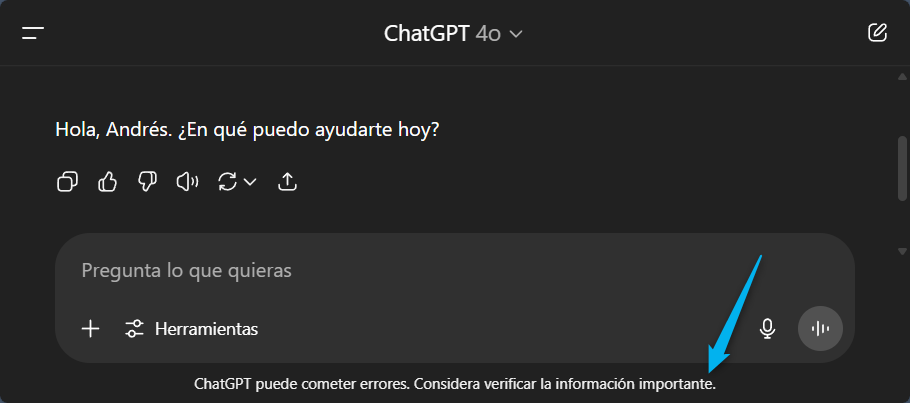
\includegraphics[width=0.8\linewidth]{Figuras/Fig01.png}
        \end{center}
    % \end{columns}
    \begin{block}{}\centering\large
        ChatGPT puede cometer errores: ¿prohibimos su uso en aula o lo aprovechamos para enseñar?
    \end{block}    
\end{frame}

\begin{frame}
    \begin{block}{Objetivo de la charla}
        \begin{itemize}[leftmargin=*]
            \item Reflexionar sobre el funcionamiento de ChatGPT y su tendencia a generar respuestas incorrectas.
            \item Presentar una experiencia concreta en el aula donde las alucinaciones se usaron como recurso didáctico.
            \item Explorar el diseño de GPTs personalizados que inducen errores con fines pedagógicos.
        \end{itemize}
    \end{block}

    \vspace{0.3cm}
    \pause
    \begin{block}{}\centering
        Caso de uso: Cálculo Diferencial
    \end{block}
\end{frame}




%%%%%%%%%%%%%%%%%%%%%%%%%%%%%%%%%%%%%%%%%%%%%%%%%%%%%%%%
\fondo{celeste}
\section{¿Cómo funciona ChatGPT?}
\fondo{blanco}
%%%%%%%%%%%%%%%%%%%%%%%%%%%%%%%%%%%%%%%%%%%%%%%%%%%%%%%%


%%%%%%%%%%%%%%%%%%%%%%%%%%%%%%%%%%%%%%%%%%%%%%%%%%%%%%%%
\begin{frame}{¿Cuál es la próxima palabra?}

\begin{center}
\begin{tikzpicture}[>=Stealth, font=\sffamily]

% Nodo principal
\node[draw, rounded corners, fill=white, minimum height=1cm, text width=3.5cm, align=center] (contexto) {El niño fue al};

% Coordenadas de destinos
\coordinate (out) at ($(contexto.east)+(1.5,0)$);

\coordinate (cafe)     at ($(out)+(1, 2.1)$);
\coordinate (hospital) at ($(out)+(1, 1.05)$);
\coordinate (parque)   at ($(out)+(1, 0)$);
\coordinate (escuela)  at ($(out)+(1, -1.05)$);
\coordinate (banco)    at ($(out)+(1, -2.1)$);

% Textos
\node[anchor=west, text=green!60!black]  at (cafe)     {\textbf{\textcolor{green!70!black}{Café}}};
\node[anchor=west, text=blue!80!black]   at (hospital) {\textbf{\textcolor{blue!80!black}{Hospital}}};
\node[anchor=west, text=violet]          at (parque)   {\textbf{\textcolor{violet}{Parque}}};
\node[anchor=west, text=red]             at (escuela)  {\textbf{\textcolor{red}{Escuela}}};
\node[anchor=west, text=brown!70!black]  at (banco)    {\textbf{\textcolor{brown!70!black}{Banco}}};

% Flechas en forma de L
\draw[->] (contexto.east) -- ++(1.5,0) |- (cafe);
\draw[->] (contexto.east) -- ++(1.5,0) |- (hospital);
\draw[->] (contexto.east) -- ++(1.5,0) |- (parque);
\draw[->] (contexto.east) -- ++(1.5,0) |- (escuela);
\draw[->] (contexto.east) -- ++(1.5,0) |- (banco);

\end{tikzpicture}
\end{center}
\end{frame}
%%%%%%%%%%%%%%%%%%%%%%%%%%%%%%%%%%%%%%%%%%%%%%%%%%%%%%%%

%%%%%%%%%%%%%%%%%%%%%%%%%%%%%%%%%%%%%%%%%%%%%%%%%%%%%%%%
\begin{frame}{¿Cuál es la próxima palabra?}

\begin{center}
    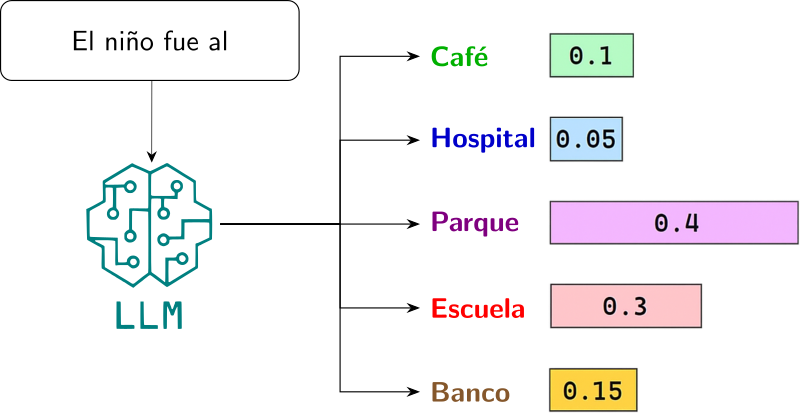
\includegraphics[width=0.8\linewidth]{Figuras/Fig03.png} 
\end{center}
\end{frame}
%%%%%%%%%%%%%%%%%%%%%%%%%%%%%%%%%%%%%%%%%%%%%%%%%%%%%%%%



%%%%%%%%%%%%%%%%%%%%%%%%%%%%%%%%%%%%%%%%%%%%%%%%%%%%%%%%
\begin{frame}{¿Cómo funciona ChatGPT?}
\begin{columns}
\column{0.7\textwidth}
\begin{block}{}
\begin{itemize}
    \item ChatGPT es una herramienta que usa los Modelos GPT de OpenAI.
    \item Los modelos GPT de OpenAI son \textbf{ modelos grandes de lenguaje} (\textit{Large Language Model}, LLM).
    \item Su tarea principal es predecir la \textbf{palabra más probable} dada una secuencia anterior.
    \item No comprende el significado, solo calcula probabilidades a partir de patrones lingüísticos aprendidos.
\end{itemize}
\end{block}
\column{0.3\textwidth}

\includegraphics[width=0.9\linewidth]{Figuras/Fig04.png} 
\end{columns}
\end{frame}
%%%%%%%%%%%%%%%%%%%%%%%%%%%%%%%%%%%%%%%%%%%%%%%%%%%%%%%%


%%%%%%%%%%%%%%%%%%%%%%%%%%%%%%%%%%%%%%%%%%%%%%%%%%%%%%%%
\begin{frame}[t]{Predicción de la siguiente palabra}
\begin{columns}
\column{0.3\textwidth}
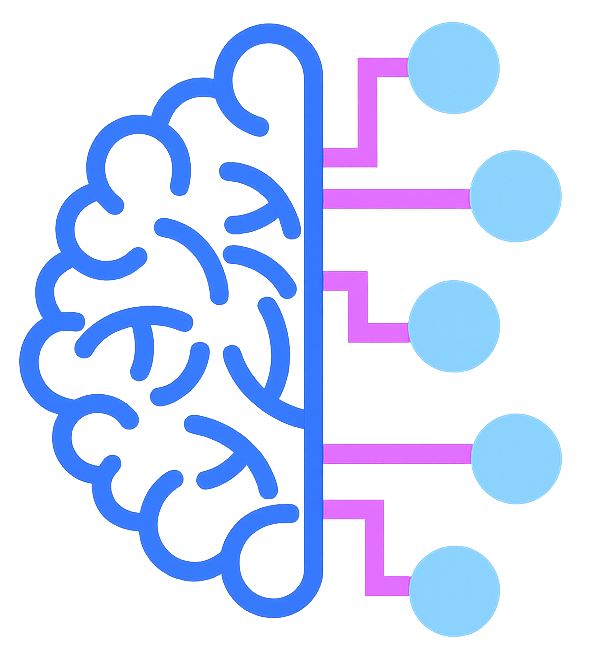
\includegraphics[width=0.9\linewidth]{Figuras/Fig05.png} 
\column{0.7\textwidth}
\begin{block}{}
\begin{itemize}
    \item El modelo asigna una \textbf{distribución de probabilidades} a cada posible palabra siguiente.
    \item No elige al azar: selecciona las opciones con mayor probabilidad.
    \item Por eso puede generar respuestas coherentes... o también \textbf{erróneas} de manera convincente.
\end{itemize}
\end{block}
\end{columns}
\end{frame}
%%%%%%%%%%%%%%%%%%%%%%%%%%%%%%%%%%%%%%%%%%%%%%%%%%%%%%%%


\begin{frame}[t]{¿Cómo se entrenó ChatGPT?}
\begin{itemize}
    \item GPT-3 fue entrenado con más de \textbf{300 mil millones de tokens} ($\sim $570 GB de texto limpio).
    \item Para GPT-4 se utilizó un volumen mucho mayor, aunque OpenAI no ha revelado cifras exactas.
\end{itemize}

\vspace{0.3cm}
\begin{block}{Fuentes principales}
\begin{itemize}
    \item \textbf{Common Crawl} (filtrado y depurado).
    \item \textbf{WebText2}, \textbf{Books1}, \textbf{Books2}, y \textbf{Wikipedia en inglés}.
\end{itemize}
\end{block}
\end{frame}
%%%%%%%%%%%%%%%%%%%%%%%%%%%%%%%%%%%%%%%%%%%%%%%%%%%%%%%%
\fondo{celeste}
\section{¿Qué son las alucinaciones en IA?}
\fondo{blanco}
%%%%%%%%%%%%%%%%%%%%%%%%%%%%%%%%%%%%%%%%%%%%%%%%%%%%%%%%

\begin{frame}[t]{¿Qué es una alucinación en IA?}

\vspace{-9mm}
\begin{columns}
\column{0.5\textwidth}
\begin{block}{Definición}
    En inteligencia artificial, una \textbf{alucinación} es una respuesta generada por un modelo que es \textbf{falsa o incorrecta}, pero expresada con gran seguridad, y que \textbf{no se justifica en los datos de entrenamiento}.
\end{block}
\column{0.5\textwidth}
\postitimg[0.9\linewidth]{Figuras/Fig06.png} 
\end{columns}
\end{frame}



\begin{frame}
\begin{block}{Ejemplos comunes}
\begin{itemize}
    \item \textbf{Errores fácticos}: datos inventados o fechas incorrectas.
    \item \textbf{Errores conceptuales}: definiciones mal formuladas.
    \item \textbf{Errores matemáticos}: pasos equivocados en cálculos o demostraciones.
    \item \textbf{Invención de fuentes}: citas o autores que no existen.
\end{itemize}
\end{block}

\vspace{0.3cm}
\pause
\begin{block}{Riesgo}
El lenguaje fluido puede ocultar el error y generar una falsa sensación de autoridad.
\end{block}
\end{frame}

\begin{frame}
    \frametitle{¿Qué tan común son las alucinaciones?}
    \centering
    \postitimg[0.6\linewidth]{Figuras/Fig11.png}
\end{frame}


\begin{frame}[t]{Potencial didáctico de las alucinaciones}
\begin{block}{¿Por qué usarlas en el aula?}
\begin{itemize}
    \item Fomentan el \textbf{pensamiento crítico} y la actitud de verificación.
    \item Permiten ejercicios de \textbf{análisis y depuración de errores}.
    \item Estimulan la \textbf{discusión argumentada} sobre conceptos.
    \item Refuerzan la comprensión al contrastar respuestas correctas e incorrectas.
\end{itemize}
\end{block}

\vspace{0.3cm}
\pause
\begin{block}{En resumen}
Una alucinación bien dirigida puede convertirse en una herramienta de aprendizaje profundo.
\end{block}
\end{frame}

%%%%%%%%%%%%%%%%%%%%%%%%%%%%%%%%%%%%%%%%%%%%%%%%%%%%%%%%
\fondo{celeste}
\section{Caso de uso}
\fondo{blanco}
%%%%%%%%%%%%%%%%%%%%%%%%%%%%%%%%%%%%%%%%%%%%%%%%%%%%%%%%

%%%%%%%%%%%%%%%%%%%%%%%%%%%%%%%%%%%%%%%%%%%%%%%%%%%%%%%%
\begin{frame}
    \frametitle{Caso de uso}

    \begin{itemize}
        \item \textbf{Asignatura:} Cálculo Diferencial e Integral
        \item \textbf{Carrera:} Ciencia de Datos
        \item \textbf{Nivel:} Segundo nivel
        \item \textbf{Trabajo:} Artículo titulado \textit{¿ChatGPT sabe Cálculo diferencial?}
        \item \textbf{Objetivo:} Evaluar las respuestas de ChatGPT sobre la historia y los procedimientos del cálculo diferencial.
    \end{itemize}
\end{frame}

%%%%%%%%%%%%%%%%%%%%%%%%%%%%%%%%%%%%%%%%%%%%%%%%%%%%%%%%

%%%%%%%%%%%%%%%%%%%%%%%%%%%%%%%%%%%%%%%%%%%%%%%%%%%%%%%%
\begin{frame}
    \frametitle{Diseño de la actividad}

    \small
    \begin{enumerate}[leftmargin=*, label=\arabic*.]
        \item Interrogar a ChatGPT sobre la historia del Cálculo desde dos cuentas distintas.
        \item Evaluar la veracidad de las respuestas con bibliografía académica.
        \item Solicitar a ChatGPT la resolución de ejercicios, incluyendo, entre otras:
        \begin{itemize}
            \item Derivada por definición
            \item Reglas de derivación
        \end{itemize}
        \item Verificar si las respuestas son correctas o contienen errores.
        \item Justificar cada error identificado y reflexionar sobre su origen.
        \item Presentar todo en un artículo estructurado, con citas y conclusiones.
    \end{enumerate}
\end{frame}

%%%%%%%%%%%%%%%%%%%%%%%%%%%%%%%%%%%%%%%%%%%%%%%%%%%%%%%%

%%%%%%%%%%%%%%%%%%%%%%%%%%%%%%%%%%%%%%%%%%%%%%%%%%%%%%%%
\begin{frame}
\centering
    \postitimg[0.6\linewidth]{Figuras/Fig07.png}
\end{frame}
%%%%%%%%%%%%%%%%%%%%%%%%%%%%%%%%%%%%%%%%%%%%%%%%%%%%%%%%

%%%%%%%%%%%%%%%%%%%%%%%%%%%%%%%%%%%%%%%%%%%%%%%%%%%%%%%%
\begin{frame}
\begin{columns}
\column{0.45\textwidth}
\begin{block}{}
    Los estudiantes «calificaron» las respuestas de ChatGPT.
\end{block}
\column{0.55\textwidth}
\centering
    \postitimg[0.95\linewidth]{Figuras/Fig08.png}
\end{columns}

\end{frame}
%%%%%%%%%%%%%%%%%%%%%%%%%%%%%%%%%%%%%%%%%%%%%%%%%%%%%%%%


%%%%%%%%%%%%%%%%%%%%%%%%%%%%%%%%%%%%%%%%
\begin{frame}{Hallazgos}
\begin{columns}
    \column{0.65\linewidth}
    \begin{itemize}[leftmargin=*]
        \item Los estudiantes demostraron alta \textbf{capacidad para identificar} y analizar errores.
        \item Detectaron \textbf{correlación} entre la \textbf{complejidad} de los ejercicios y la \textbf{precisión} de ChatGPT.
        \item Se fomentó el \textbf{pensamiento crítico} y la comprensión profunda de los conceptos matemáticos.
    \end{itemize}
    \column{0.35\linewidth}
    \postitimg[0.98\linewidth]{Figuras/Fig09.png}
\end{columns}
\end{frame}

%%%%%%%%%%%%%%%%%%%%%%%%%%%%%%%%%%%%%%%%%%%%%%%%%%%%%%%%
\fondo{celeste}
\section{GPTs para errores intencionados}
\fondo{blanco}
%%%%%%%%%%%%%%%%%%%%%%%%%%%%%%%%%%%%%%%%%%%%%%%%%%%%%%%%

\begin{frame}
    \frametitle{La IA mejora: menos alucinaciones}

    \centering
    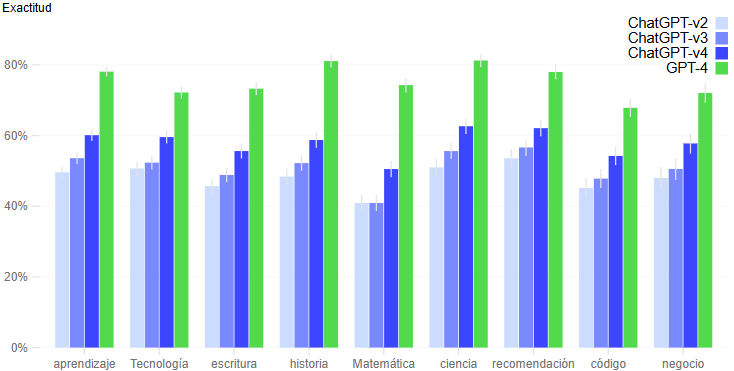
\includegraphics[width=0.85\linewidth]{Figuras/Fig10.png}
\end{frame}


\begin{frame}
    \frametitle{¿Y si la IA ya no alucina?}

    \begin{itemize}
         \item Modelos recientes, como \textbf{GPT-4}, muestran una mejora significativa en la exactitud de sus respuestas.
        \item Esta mejora \textbf{reduce las alucinaciones}, pero también limita los casos espontáneos útiles para el aprendizaje crítico.
        \item \textbf{¿Cómo conservar el valor didáctico de las alucinaciones si la IA deja de cometerlas?}
    \end{itemize}
\end{frame}


\begin{frame}

     Se creó un GPT personalizado llamado  \href{https://chatgpt.com/g/g-6853670f47648191917d013f9d97448c-derivador-3000}{\textbf{Derivador 3000}}.

    \centering
    \postitimg[0.8\linewidth]{Figuras/Fig12.png}\\\footnotesize
    \url{https://chatgpt.com/g/g-6853670f47648191917d013f9d97448c-derivador-3000}
\end{frame}

\begin{frame}


    Está diseñado para cometer \textbf{errores sutiles y esporádicos} en derivación.


    \centering
    \postitimg[0.85\linewidth]{Figuras/Fig13.png}
\end{frame}


%%%%%%%%%%%%%%%%%%%%%%%%%%%%%%%%%%%%%%%%%%%%%%%%%%%%%%%%
\fondo{celeste}
\section{Conclusiones}
\fondo{blanco}
%%%%%%%%%%%%%%%%%%%%%%%%%%%%%%%%%%%%%%%%%%%%%%%%%%%%%%%%

%%%%%%%%%%%%%%%%%%%%%%%%%%%%%%%%%%%%%%%%%%%%%%%%%%%%%%%%
\begin{frame}
    \frametitle{Conclusiones}

    \begin{itemize}
        \item El uso pedagógico de las alucinaciones de ChatGPT \textbf{potenció el análisis crítico} en el aula.
        \item Los estudiantes aprendieron a \textbf{dudar de las respuestas automáticas}.
        \item Se promovió la \textbf{verificación con fuentes oficiales} y el contraste riguroso de la información.
    \end{itemize}

    \pause
    \vspace{0.4cm}
    \begin{block}{}
    Convierte los errores de la IA en aliados del aprendizaje. \textbf{¡Replica esta experiencia en tu asignatura!}
    \end{block}
\end{frame}




%%%%%%%%%%%%%%%%%%%%%%%%%%%%%%%%%%%%%%%%
%% Página final
\fondo{final}
\begin{frame}[plain]
\begin{center}
    \color{white}
    
    \vspace{1.5cm}
    {\Huge\textbf{Gracias}}
    \vspace{2mm}
    

    \begin{tabular}{ccc}
        \textcolor{azul}{\qrcode[height=3cm]{https://linktr.ee/aemerinot}}
        &
        \phantom{.\hspace{.5cm}.}
        &
        \textcolor{azul}{\qrcode[height=3cm]{https://andres-merino.github.io/Presentacion-ChatGPT-DidacticaAlucinaciones/DidacticaAlucinaciones.pdf}}
        \\ \\[-2mm]
        \LARGE \faLinkedin\hspace{5mm} \faGithub%\hspace{5mm} \aiOrcidSquare 
        && 
        Presentación
    \end{tabular}\\
    \vspace{2mm}
    \textbf{Contacto:} aemerinot@puce.edu.ec
\end{center}
\end{frame}


\end{document}